\subsection{Projects}
The point is to have two applications that are similar. This way we can see if the SDS brings improvements for the user. For this reason, it is important that both systems are visually indistinguishable from each other. Both systems consist of three views and an optional view that is used to explain the test case task to the user. Therefore, this view is omitted from the count. \\

\begin{figure}[hbtp]
    \centerline{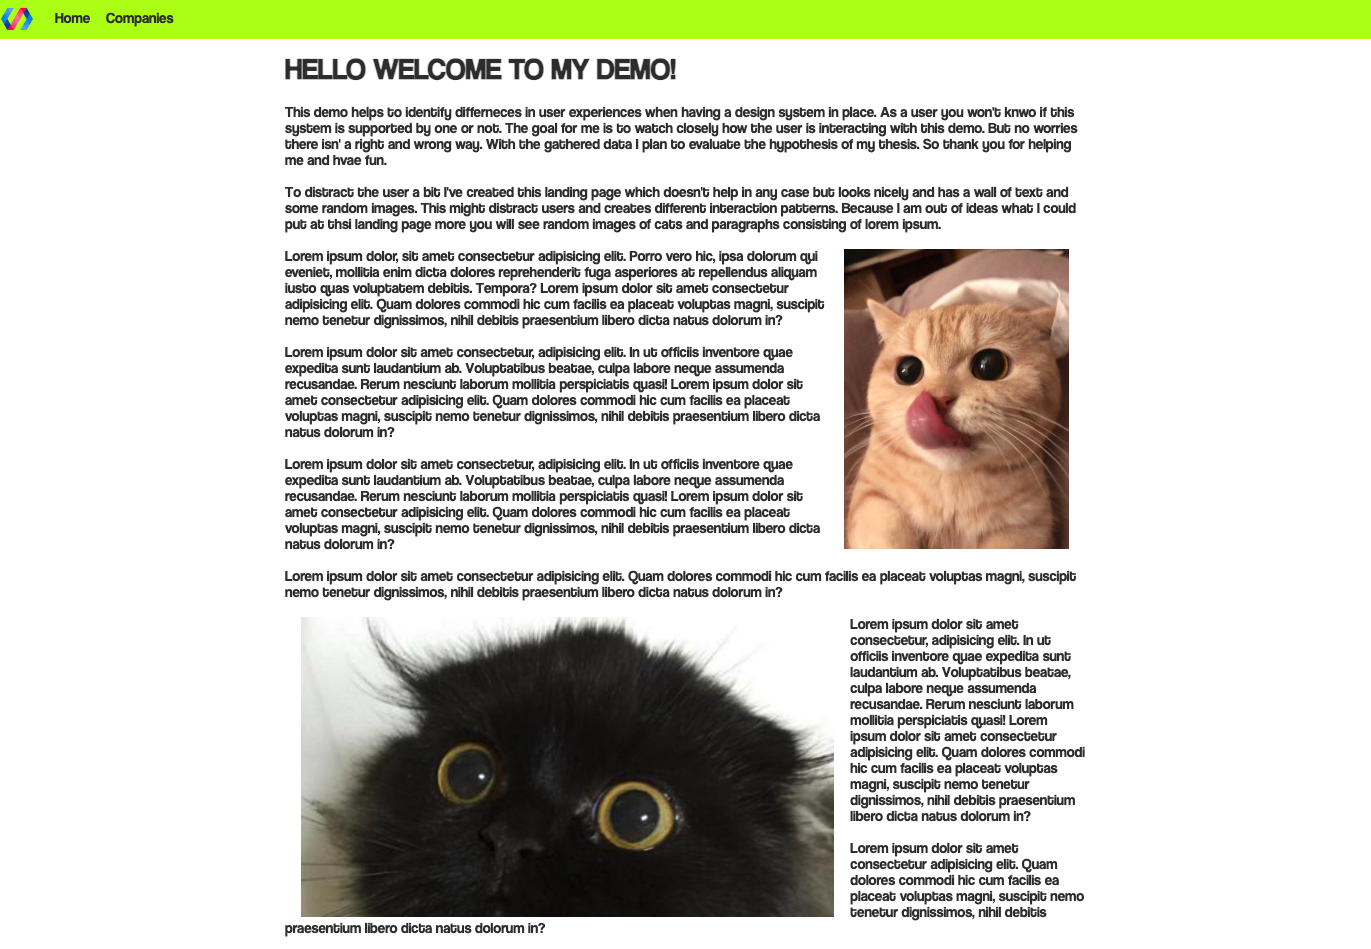
\includegraphics[width=\linewidth, draft=false]{images/demo_view_landing_page.png}}
    \caption{Landing page of test applications}
    \label{landing_page}
    \end{figure}
The first view (Figure \ref{landing_page}) is the landing page when the user starts the test run. Here the user will find a navigation bar, which is also included in the other two views, to navigate through the application. The main goal of this view is to distract the user. Long paragraphs with sample texts and cat photos are meant to draw the user away. After all, he is supposed to navigate to the second view, the data table, via the upper navigation bar. When the user clicks on "Company", he is redirected to the second view. 
\\

In the second view (Figure \ref{data_table}), the user sees a data table with entries from various made-up companies. Besides the company name, the user finds the current status of the company and a description in the table. The description is also a Lorem ipsum without any relevance. At the top right of the data table, the user finds a button labelled "Add +". This button leads him to the third view. 
\begin{figure}[htbp]
    \centerline{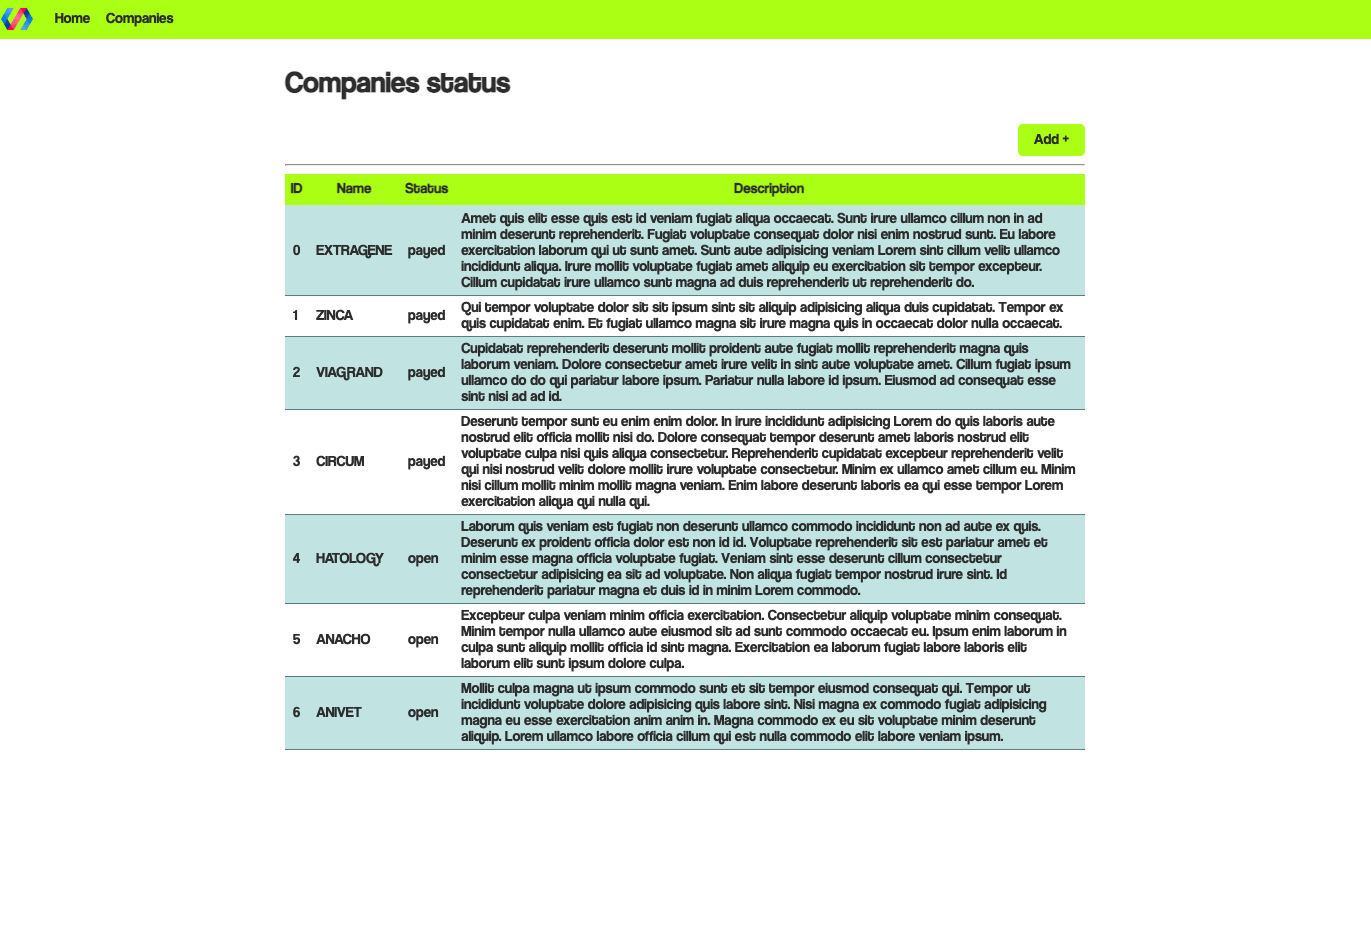
\includegraphics[width=\linewidth, draft=false]{images/demo_view_data_table.png}}
    \caption{Data table page of test applications}
    \label{data_table}
    \end{figure}
    \\

The last view (Figure \ref{adding_form}) of the sample applications shows a form for adding new data to the table. The form has three inputs for each value corresponding to the table from the second view. All inputs are plain text inputs with no restriction or validation of the inputs. In a real scenario, there would be validation, but due to the limited time frame of this elaboration, this feature is omitted. At the bottom of the form, the user sees a button to save the form. This button is disabled until all input fields are filled with a value. 
\begin{figure}[htbp]
    \centerline{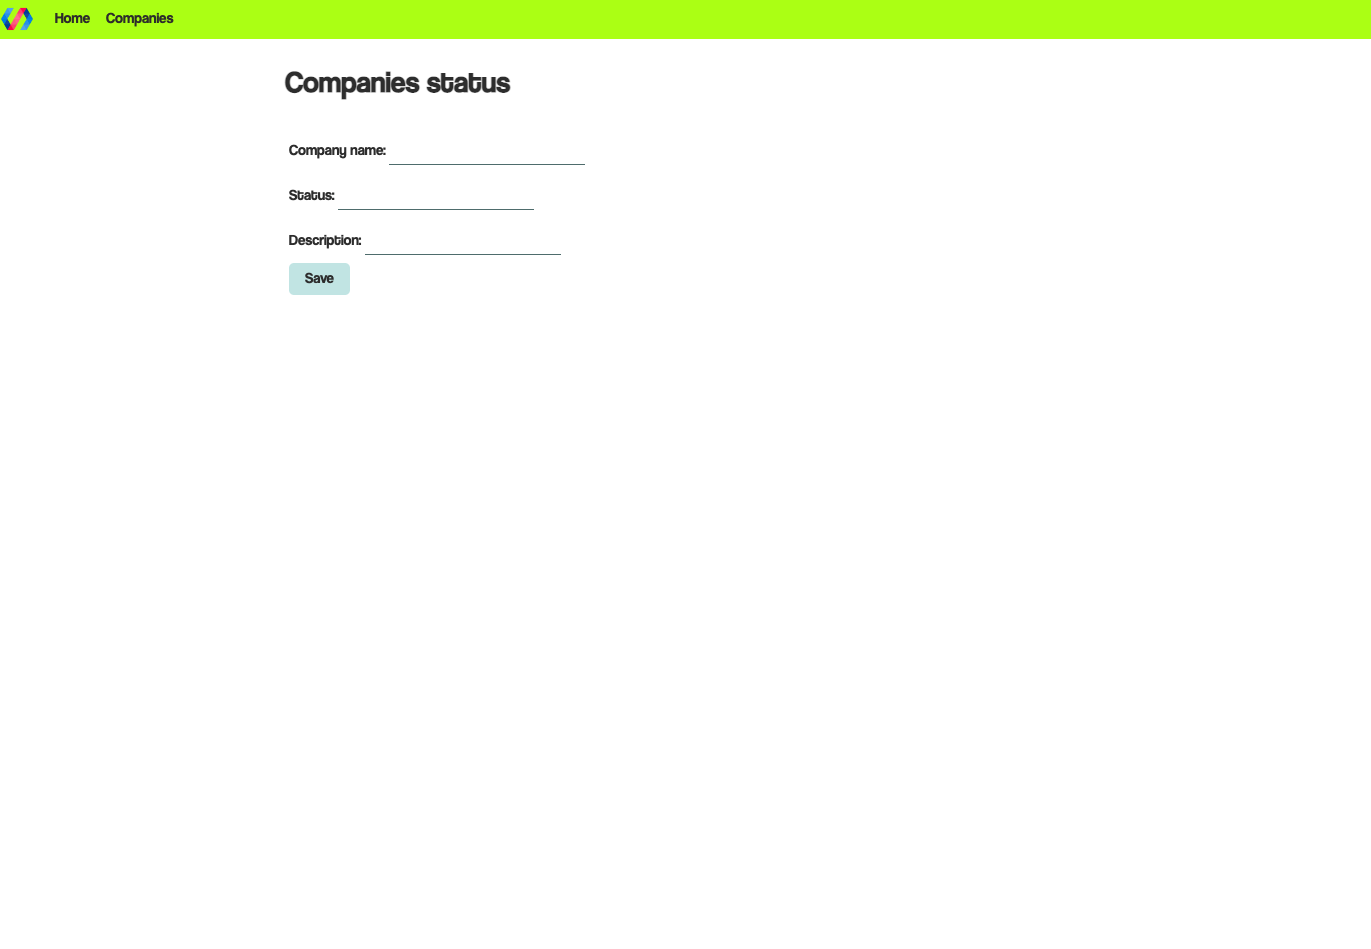
\includegraphics[width=\linewidth, draft=false]{images/demo_view_form.png}}
    \caption{Data adding view of test applications}
    \label{adding_form}
    \end{figure}
\\

Both applications not only have the same views, but also the same technology stack. They are based on Svelte, a library for building web applications with a small package size. According to the starter guide, we use Rollup as a bundling and compilation tool. So both applications do not differ in terms of technology and build steps. \cite{svelte_svelte_nodate} \\
The only difference between the two systems are the implementation details. The next chapters will therefore explain the structure of each application and how views are created with and without SDS.
\subsubsection{Application using \ac{SDS}}
First, a summary of how to use the \acl{SDS}. To use the web components, the application must import the code that adds the components. In this case, the system contains the bundle described in \ref{SDS_build_and_integration}. This is done via the \texttt{main.ts} file, which is defined as an input file in the rollup configuration. \\
\lstinputlisting[linerange={1-9},firstnumber=1,caption={Bootstrapping of Svelte application with \ac{SDS}},label=BootstrappingAppSDS]{../Code/sds-demo-app/src/main.ts}
As can be seen in Listing \ref{BootstrappingAppSDS}, the bootstrapping of the Svelte application is performed here by creating the Svelte App component and appending it to the body. Also, in line 2 and 3, the SDS bundle Javascript and CSS is imported. This adds the design system components and its styles to the application. Now it is possible to use all the web components within the app via the HTML tags defined by \ac{SDS}. \\

After successfully bootstrapping the app, the next step is to look at the Svelte components themselves and how they build the given views. Since the app component is only needed for bootstrapping and initialising the router, another check can be omitted. According to the routing details, the next component to be loaded is Main.svelte. \\
The Main component is responsible for displaying the navigation bar, which can be seen at the top of each displayed view. In addition, it contains a content placholder where other components are displayed. The code of the component shows that web components from the \ac{SDS} are used. Line 7-11 in Listing \ref{MainSvelteSDS} use the navigation bar (\texttt{<saas-navbar>}) and the corresponding navigation bar items (\texttt{<saas-navbar-item>}).
\lstinputlisting[linerange={1-14},firstnumber=1,caption={Main.svelte with \ac{SDS}},label=MainSvelteSDS]{../Code/sds-demo-app/src/components/Main.svelte}
The component takes advantage of the functionality of slots by inserting elements into the navbar component. The web component then takes care of the corresponding display at the top. The Navbar elements inside ensure that the declared navigation links are displayed with the correct styles defined by the design system. A special feature in line 8, Listing \ref{MainSvelteSDS} is the \texttt{<img>} element. This HTML element is responsible for displaying the logo in the upper left corner. The element has a special property called "slot". Its value is set to "logo". The web component of the navigation bar recognizes this slot definition and inserts the image with the expected styles in the navigation bar. \\
Below the code for the navigation bar, lines 12-14, Listing \ref{MainSvelteSDS} contain the code for displaying the content of the application. In addition to the navigation bar web component, the content web component is also provided with the design system. It uses the same logic as the navigation bar by providing a placeholder for elements within that component and applying styles to the content container within the web component. Adjustable by design token within the SDS. The \texttt{<Router>} tag within the content is an imported Svelte component that handles the display of the content according to the visited route. \\
One route that is visited at the beginning of the test is the landing page. The page is represented by the Svelte component \texttt{Home.svelte}. This component consists only of a few paragraphs and images to distract the user. Therefore, it is not necessary to go into details here. The final result of the view can be seen in Figure \ref{landing_page}.\\
An important component in this comparison is Data.svelte. As the name suggests, this component manages the view of the data table shown in Figure \ref{data_table}. However, not only the view of the data table is managed here, but also the view of the data entry form shown in Figure \ref{adding_form} can be seen in the component's code. \\
\lstinputlisting[linerange={84-90},firstnumber=84,caption={Data.svelte with \ac{SDS} table implementation},label=DataSvelteSDSTable]{../Code/sds-demo-app/src/components/Data.svelte}
SDS provides a web component for data tables. The component is used in line 89 in Listing \ref{DataSvelteSDSTable}. To display the data in the table, two properties must be set. The \texttt{header} property, as the name implies, manages the headers that are displayed in the table. The \texttt{hedaer} object defines a mapping of keys of the table data to the string values that will be displayed as table headers. Accordingly, the second property is the data input for the table. The data object \texttt{myArray} is put into the \texttt{data} property of the table web component. The data structure of the array should match the data keys defined in the header object so that the data objects within the array match the table headers. \\
Figure \ref{data_table} shows a button at the top of the table. The button is also added in this code snippet. Lines 85-87 show the code where the button is added. As with the table component, the design system provides a button component that was introduced in Section \ref{sds_button}. The \texttt{on:click} property is an indicator of an event listener in Svelte. In this case, a click listener. The event property is connected to the \texttt{addEntry} function within the Data.svelte component. This function simply toggles the boolean variable \texttt{isAddEntry} to \texttt{true}. When the variable is changed, the if statement on line 84 is \texttt{false} and activates the else block at line 90. \\

Like described in the flow above, the else block consists of elements to create the view of Figure \ref{adding_form}, the form view. The code snippet looks like this:
\lstinputlisting[linerange={90-100},firstnumber=90,caption={Data.svelte with \ac{SDS} form implementation},label=DemoSvelteSDSForm]{../Code/sds-demo-app/src/components/Data.svelte}
The standard form element between lines 91 and 99 contains the form inputs and a "Save" button. Like the table and the buttons, the form input fields are web components of the design system. The inputs have custom properties for setting the label and its ID to ensure appropriate accessibility. A special feature of this web component is the custom event for a value change. For example, in line 92 Listing \ref{DemoSvelteSDSForm}, the input receives an event object through this value event and deconstructs the event object to access its details. These details include the changed value of the input field. This value is then assigned to the newly created data object. \\
After all input fields have set a value in the new data object. The "Save" button changes its property \texttt{disbaled} to \texttt{false} and allows click events for itself. With a final click on the button, the freshly created object is then attached to the data table array and appears on the bottom. This shows all the possibilities of the first test system and the other variant without using the SDS can be explained in the next section.

\subsubsection{Application not using \ac{SDS}}
One of the main goals is to have a similar application with the same capabilities, but not using the design system. So it is necessary to recreate the application from the previous section without using its components. \\
In order not to have major technical differences, this application uses the same technical stack as the first demo system. So the bootstrapping of the application looks the same as in Listing \ref{MainSvelteSDS}, but without the import of SDS code and styles. The application runs and uses Svelte components to create the views described above. \\

As before, a detailed look at the App.svelte is not necessary, as it is only where the routing for the Single Page Application is initialized. The first code to look at is in the Main.svelte component to see how the navigation bar and router content is constructed in this type of application. 
\lstinputlisting[linerange={1-17},firstnumber=1,caption={Main.svelte without \ac{SDS}},label=MainSvelteNormal]{../Code/normal-demo-app/src/components/Main.svelte}
Besides using fewer lines of code compared to Listing \ref{MainSvelteSDS}, the main difference is that no custom web components are used for the navigation bar or elements. Here, web standards are followed by using the correct HTML tags to describe specific areas of the application. \\
For example, the navigation bar uses the \texttt{<nav>} tag in lines 6-12 to enclose an unsorted list that tells the browser that this is a navigation area for the application. The same construct of an HTML tree was used in the \ac{SDS} demo, but hidden behind web components so the developer doesn't have to think about it when implementing a navigation bar. \\
The same concept can be seen below the navigation bar code in lines 13-17, Listing \ref{MainSvelteNormal}. Here the main content is encapsulated by a \texttt{<main>}, which is also an indicator for the browser. \\
But the part that is not visible in Listing 11 and must be added to get a proper look for this HTML element is the styling. Since the SDS components are built based on best practices from across the field, no one has to develop a new styling concept and fix style glitches that may occur during development. 
\lstinputlisting[linerange={18-48},firstnumber=18,caption={Main.svelte styles without \ac{SDS}},label=MainSvelteNormalStyles]{../Code/normal-demo-app/src/components/Main.svelte}
As seen in Listing \ref{MainSvelteNormalStyles}, many styles have fixed values for style rules. As in line 23, it is possible to define design tokens in an application and use them in place of the fixed values, but there is no guarantee that they will be used throughout the application. In an existing design system, components ensure that they are built on the defined design tokens. \\
But it's not just consistency that's important, it's also the time required to rewrite those lines of code over and over again for each new application. If something already exists, it should be used.Ultimately, this code snippet produces the same view of Figure \ref{landing_page} as in the other demo, but it takes a lot more thinking to get to this result.  \\

The demo project without using the SDS also creates the second view shown in Figure 8, the data table. For this, the project contains a svelte component with the same name, Data.svelte, as in the previous section. As in the other application, Data.svelte consists of two views simultaneously. 
Starting with the data table view, the responsible code snippet looks like this:
\lstinputlisting[linerange={86-92},firstnumber=86,caption={Data.svelte without \ac{SDS} table implementation},label=DataSvelteNormalTable]{../Code/normal-demo-app/src/components/Data.svelte}
At first glance, the component code looks quite similar to that in Listing \ref{DataSvelteSDSTable}. But the names of the \texttt{<SvelteTable>} table component and the \texttt{<SvelteButton>} button component give a hint of how these components are constructed. Both are Svelte components that replicate the logic familiar from the Web components presented earlier. \\
One might say, why then should it be necessary to build web components when it is also possible to build them this way and ensure no style inconsistencies. The answer is that this works for an application with this specific technology stack to reuse these Svelte components. If one is okay with using a limited technology stack to ensure the use of a specific component library, then that's fine. But the reality is that there are many different frameworks, each with a specific component implementation.\\
In this case, the application builds each component itself and uses it here, as shown in lines 88 and 91 in Listing \ref{DataSvelteNormalTable}. 
The button in the upper right is represented by the \texttt{<SvelteButton>} element and receives an event to switch to the third view, the form view. Because it is a standalone component, the styles for the button are not in the code for the Data.svelte component, but in the code (Listing \ref{SvelteNormalButton}) for the button. As explained with the navigation bar, the button styles are defined as fixed values, not as design tokens that would be provided by a design system. This causes difficulties when changing the appearance of multiple components with a single value change. \\
The same rules apply to the table component just presented. Both properties are responsible for ending up with the table from Figure \ref{data_table} as the render result. This sets up the second view and a click on the button reveals the third view (Figure \ref{adding_form}). \\

To conclude the implementation details of the second demo application that does not use the SDS, it is time to take a look at the code that creates the form for entering a new data object into the table. As before, these elements are visible if the if statement from line 86, Listing \ref{DataSvelteNormalTable} results in a \texttt{false} statement, ergo \texttt{isAddEntry} is \texttt{true}. This is the block of code that displays the input fields in the browser:
\lstinputlisting[linerange={92-99},firstnumber=92,caption={Data.svelte without \ac{SDS} form implementation},label=DataSvelteNormalForm]{../Code/normal-demo-app/src/components/Data.svelte}
A new svelte component can be seen in lines 94-96, Listing \ref{DataSvelteNormalForm}. This component, as the name <SvaleteInput> indicates, is a text input field for the form. In addition to the familiar property of indicating an input by specifying a string value, there is a special Svelte property. The keyword \texttt{bind} indicates a two-way data binding in Svelte. This means that the assigned value is stored in the component and that if this variable is changed within the component, the changes are reflected back in the object value.\\  
Recalling the code snippet from the web component implementation (Listing \ref{DemoSvelteSDSForm}), it is not possible to \texttt{bind} a value and the event output of a custom web component. In this case it was necessary to listen to the event manually to get the details. Whether it is worth avoiding the use of web components in frameworks because of the lack of such features can be discussed later in the conclusion. \\
With the addition of the button component in line 97, Listing \ref{DataSvelteNormalForm}, the implementation of the form to submit new data to the data field is complete. As with the web component implementation, the button has a \texttt{disabled} property that blocks click events when set to true. Validating the form's input values will either disable the button or not. \\


This concludes the details of the implementation of the demo systems used to test the SDS. The next step is to examine the test case that was planned to test the design system.
% View 3 